\documentclass[12pt, oneside]{article} 
\usepackage{amsmath, amsthm, amssymb, calrsfs, wasysym, verbatim, bbm, color,
graphics, geometry}
\usepackage[dvipsnames]{xcolor}
\usepackage[utf8x]{inputenc} % Включаем поддержку UTF8
\usepackage[T2A]{fontenc}
\usepackage[english, russian]{babel}
\usepackage{hyperref}
\usepackage{tikz}
\usepackage{wrapfig}
\usepackage{bm}
\numberwithin{equation}{section}  % Формулы нумеруются как (X.Y), где X — номер раздела


\geometry{tmargin=.75in, bmargin=.75in, lmargin=.75in, rmargin = .75in}  


\newtheorem{thm}{Theorem}
\newtheorem{defn}{Definition}
\newtheorem{conv}{Convention}
\newtheorem{rem}{Remark}
\newtheorem{lem}{Lemma}
\newtheorem{cor}{Corollary}


\title{\huge Квантово-химическое моделирование молекулярных систем\\ \rule{0.8\textwidth}{0.4pt} \\ \large \textit{курс лекций}}

\date{2025г}

\begin{document}

\maketitle
\tableofcontents

\vspace{.25in}

\section{Многоэлектронные волновые функции и операторы}

\subsection{Постановка задачи. Атомные единицы. Многоэлектронная проблема}


\hspace{0.4cm} Нашей задачей является нахождение решений стационарного уравнения Шрёдингера в нерелятивстском приближении

\begin{equation}
    \hat{H} |\psi \rangle = E | \psi \rangle
    \label{eq:Shr}
\end{equation}

В СГС для атома водорода:

\begin{equation}
    \left[ - \dfrac{\hbar^2}{2 m_e} \nabla^2 - \dfrac{e^2}{r}\right] \psi = E \psi
\end{equation}


Чтобы обезразмерить данное уравнение в атомных единицах принято полагать: \(m_e = 1, e = 1, \hbar = 1\) (скорость света тогда равна обратной постоянной тонкой сктруктуры)
\begin{equation}
    \left[- \dfrac{1}{2} \nabla^2 - \dfrac{1}{r} \right] \psi = E \psi
\end{equation}
Энергия атома водорода в таком случае равна \(- \dfrac{m e^4}{2 \hbar^2} = - 0.5\) ед. Хартри \( = -13.6\) эВ.

В случае нескольких ядер и электронов:

\begin{equation}
    \psi = \psi(\bm{R}_1, \dots, \bm{R}_K, \bm{r}_1, \dots, \bm{r}_N, \sigma_1, \dots, \sigma_N)
\end{equation}


Для молекулы воды возникает 43 независимых координаты, поэтому сетка параметров в 100 точек на каждой координате приведёт к общему числу точек: \(100^{43} = 10^{86}\), что не позволяет решать уравнение численно.

Решать систему дифференциальных уравнений можно несколькими способами:

1) Функции Грина. Например, метод GW. Хорошо предсказывает bandgap, используется для твердого тела и молекул.

2) Метод рядов Фурье \(\psi = \sum_k c_k \phi_k\). Такой ортогональный базис можно получить через детерминанты Слейтера, о чём будет сказано далее.


Покажем основные обозначения для компонент гамильтониана:

\begin{equation}
    \hat{H} = \hat{T} + \hat{V} = \hat{T}_n + \hat{T}_e + \hat{V}_{ne} + \hat{V}_{ee} + \hat{V}_{nn}
\end{equation}
где 


\begin{gather}
\label{eq:kin}
\hat{T}_n = - \frac{1}{2} \sum \frac{1}{M_\alpha} \nabla_\alpha^2,\; \hat{T}_e = - \frac{1}{2} \sum \nabla_i^2 \\
\hat{V}_{nn} = \sum_{\alpha < \beta} \frac{Z_\alpha Z_\beta}{|\vec{R}_\alpha - \vec{R}_\beta|} \;
\hat{V}_{ne} = - \sum_{\alpha, i} \frac{Z_\alpha}{|\vec{R}_\alpha - \vec{r}_i|} \;
\hat{V}_{ee} = \sum_{i < j} \frac{1}{|\vec{r}_i - \vec{r}_j|}
\end{gather}

Помимо этого есть спин-спиновое взаимодействие (например, в уране, это взаимодействие может иметь вклад до \(5 \%\) от ответа, что очень много для расчётов в химии)

Также есть и спин-орбитальное взаимойствие (например, в органике практически нет необходимости его учитывать). Для учёта данного взаимодействия существует \textit{гамильтониан Брейта}.

Учёта выше перечисленных взаимодействий не требуется для первых двух периодов таблицы Менделеева. 

\subsection{Приближение Борна-Оппенгеймера. Поверхность потенциальной энергии}

\begin{wrapfigure}{r}{0.4\textwidth}
    \centering
    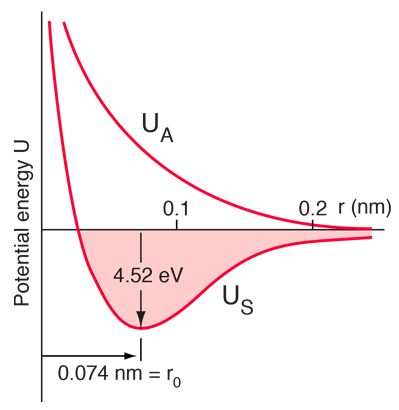
\includegraphics[width=0.3\textwidth]{./images/H2.png}
    \caption{Поверхность потенциальной энергии H\(_2\)}
    \label{fig:H2PPE}
\end{wrapfigure}
Поскольку ядра значительно тяжелее эелктронов, их движение происходит медленнее, чем у электронов. Поэтому хорошей аппроксимацией можно считать, что электроны в молекуле движутся в поле неподвижных ядер. 
Следовательно, в (\ref{eq:kin}) можно пренебречь вкладом \(\hat{T}_n\), а \(\hat{V}_{nn}\) можно считать константой, что не влияет на собственные функции гамильтониана, поэтому он приводится к виду
\begin{equation}
    \hat{H}_e = \hat{T}_e + \hat{V}_{ne} + \hat{V}_{ee} + V_{nn},
    \label{eq:H_e}
\end{equation}
Потенциал \(V_{nn}\) часто включают в гамильтониа, чтобы корректнее интерпретировать спектр с точки зрения физического смысла.
Таким образом приходим к электронному уравнению Шрёдингера

\begin{equation}
    \hat{H}_e \psi_e (\bm{r}| \bm{R} ) = E_e (\bm{R}) \psi_e (\bm{r}| \bm{R}),
\end{equation}
где положение ядер \(\bm{R}\) является параметром.



Энергия \(E_e(\bm{R})\) может быть использована как потенциал при решении задачи движения ядер. Множество её значений в зависимости от координат называется \textit{поверхностью потенцильной энергии} Её график в случае молекулы H\(_2\) указан на рисунке \ref{fig:H2PPE}. Имеется всего лишь одна координата - расстояние между ядрами, причём нижняя кривая соответствтует синглетному состоянию (\(S = 0\)), или основному состоянию для спектра электронного гамильтониана в каждой точке \(\bm{R}\), а верхняя - триплентному (\(S = 1\)). 

Стоит отметить, что хотя массы электронов и ядер отличаются на порядки (\(10^3 \div 10^5\)) имеются и случаи, когда пренебрегать такой разницей уже нельзя. Например, при исследовании лёгких веществ с помощью мюонов. Помимо этого, приближение Борна-Оппенгеймера часто предполагает большое расстояние между поверхностями потенциальной энергии, и в связи с этим приводит к невозможности системы переходить между ними. Такое, в частности, наблюдается в молекулах ретиналя, отвечающих за детектирования света клетками нашего глаза. В условиях адиабатичности они бы не могли менять конформацию.

Волновую функцию всей системы можно представить\footnote{При каждом фиксированном \(\bm{R}\) функция \(\psi(\bm{R})\) раскладывается по ортонормированному базису собственных функций электронного гамильтониана (\ref{eq:H_e}): \(\langle \psi_i | \psi_j \rangle = \delta_{ij}\).} как 

\begin{equation}
    \psi = \sum_{k=0}^{\infty} \chi_k (\bm{R}) \psi_k (\bm{r}| \bm{R})
\end{equation}
где \(\chi_k(\bm{R})\) - ядерные волновые функции


Тогда уравнение Шредингера \ref{eq:Shr} примет вид:
\begin{equation}
(\hat{T}_n + \hat{H}_e) \sum_k \chi_k (\bm{R}) \psi_k (\bm{r}| \bm{R}) = E \sum_k \chi_k (\bm{R}) \psi_k (\bm{r}| \bm{R})
\end{equation}

Домножим слева на \(\langle \psi_m|\):

\begin{equation}
\langle \psi_m | \hat{T}_n | \sum_k \chi_k \psi_k \rangle + \langle \psi_m | \hat{H}_e | \sum_k \chi_k \psi_k \rangle = E \langle \psi_m | \sum_k \chi_k \psi_k \rangle
\end{equation}

Воспользуемся ортонормированностью базиса: \(\langle \psi_m | \sum_k \chi_k \psi_k \rangle = \sum_k \chi_k \delta_{mk} = \chi_m\), а также тем, что \(\langle \psi_m | \hat{H}_e = \langle \psi_m | E_m \).

\begin{equation}
- \frac{1}{2} \sum_{k} \left[ \sum_\alpha \frac{1}{M_\alpha} \langle \psi_m |\nabla_\alpha^2 | \psi_k \chi_k \rangle \right]
+ E_m \chi_m = E \chi_m
\label{eq:shr1}
\end{equation}

Распишем лапласиан:

\[\nabla_\alpha \nabla_\alpha \chi_k \psi_k = \nabla_\alpha \left[(\nabla_\alpha \chi_k ) \psi_k + \chi_k (\nabla_\alpha \psi_k)\right] = (\nabla_\alpha^2 \chi_k ) \psi_k + 2 (\nabla_\alpha \chi_k) (\nabla_\alpha \psi_k ) + \chi_k (\nabla_\alpha^2 \psi_k)\]

Функция вида \((\nabla_\alpha \chi_k)\) зависит только от параметра \(\bm{R}\), поэтому её можно выносить из матричного элемента. В итоге слагаемое с суммой из (\ref{eq:shr1}) преобразуется так:

\begin{equation}
\begin{split}
    \sum_k \left(- \dfrac{1}{2} \sum_\alpha \dfrac{1}{M_\alpha} (\nabla_\alpha^2 \chi_k) \delta_{mk} - \sum_\alpha \dfrac{1}{M_\alpha} \langle \psi_m | \nabla_\alpha| \psi_k \rangle \nabla_\alpha \chi_k - \dfrac{1}{2} \sum_\alpha \dfrac{1}{M_\alpha} \langle \psi_m |(\nabla_\alpha^2 \psi_k) \rangle \chi_k \right) =\\
     = \underbrace{\left[- \dfrac{1}{2} \sum_\alpha \dfrac{1}{M_\alpha} \nabla_\alpha^2 \right]}_{\hat{T}_n} \chi_m - \sum_k \sum_\alpha \dfrac{1}{M_\alpha} \langle \psi_m | \nabla_\alpha | \psi_k \rangle \nabla_\alpha \chi_k - \dfrac{1}{2} \sum_k \sum_\alpha \dfrac{1}{M_\alpha} \langle \psi_m |(\nabla_\alpha^2 \psi_k) \rangle \chi_k 
\end{split}
\end{equation}

Таким образом (\ref{eq:shr1}) переходит в 

\begin{equation}
    \hat{T}_n \chi_m + E_m \chi_m - \sum_k \left[\sum_\alpha \dfrac{1}{M_\alpha} \overbrace{\langle \psi_m |\nabla_\alpha | \psi_k \rangle}^{A_{mk}} \nabla_\alpha \right] \chi_k - \dfrac{1}{2} \sum_k \left(\sum_\alpha \overbrace{\langle \psi_m | \nabla^2_\alpha | \psi_k \rangle}^{B_{mk}} \right) \chi_k = E \chi_m 
    \label{eq:shr2}
\end{equation}

Попробуем упростить данное уравнение. Рассмотрим при каких условиях можно пренебречь недиагональными матричными элементами.

Оценим \(A_{mk}\). При \(m = k\) в случае выбора вещественных волновых функций.

\[0 = \nabla_\alpha \langle \psi_m | \psi_m \rangle = 2 \langle \psi_m | \nabla_\alpha \psi_m \rangle\]

При \(m \neq k\)

\[0 = \nabla_\alpha \langle \psi_m | \hat{H}_e| \psi_k \rangle = E_k \langle \nabla_\alpha \psi_m | \psi_k \rangle + \langle \psi_m | (\nabla_\alpha \hat{H}_e) | \psi_k \rangle + E_m \langle \psi_m | \nabla_\alpha \psi_k \rangle \]

Откуда, пользуясь тем, что \(\langle \psi_m | \nabla_\alpha \psi_k \rangle = - \langle \nabla_\alpha \psi_m | \psi_m \rangle\), получаем

\begin{equation}
    A_{mk} = \langle \psi_m | \nabla_\alpha \psi_k \rangle = \dfrac{\langle \psi_m | (\nabla_\alpha \hat{H}_e )| \psi_k \rangle}{E_k - E_m}
    \label{eq:bf}
\end{equation}

Уравнение (\ref{eq:bf}) называется \textit{формулой Борна-Фока}. В случае, если \(A_{mk} \ll A_{mm}\), \(m \neq k\), что характерно для больших расстояний между энергиями \(E_k\) и \(E_m\), в уравнении (\ref{eq:shr2}) можно пренебречь слагаемыми с \(A_{mk}\), \(m \neq k\). Аналагично пренебрегаются и \(B_{mk}\), \(m \neq k\), как поправки второго порядка к неадиабатичности.

С учётом вышесказанных приближений уравнение (\ref{eq:shr2}) переходит в

\begin{equation}
    \left[ \hat{T}_n + E_m (\bm{R}) \right] \chi_m + \overbrace{\langle \psi_m | \hat{T}_n | \psi_m \rangle}^{B_{mm}} \chi_m = E \chi_m
    \label{eq:shr3}
\end{equation}

Матричный элемент \(B_{mm}\) называется диагональной Борн-Оппенгеймееровской поправкой (DBOS).
С DBOS уравнение (\ref{eq:shr3}) записано в \textit{адиабатическом приближении}. Без DBOS в \textit{приближении Борн-Оппенгеймера}:

\begin{equation}
    \left[ \hat{T}_n + E_m (\bm{R}) \right] \chi_m = E \chi_m
\end{equation}

\end{document}
